\section{Grundlegende Theorie}
\subsection{Definition}
Im weitesten Sinne beschreibt ein Buffer Overflow eine Schwachstelle in einem Computerprogramm,
bei der ein Angreifer einen Speicherbereich fester Größe überschreibt und diesen so zum “Überlaufen” bringt.
Durch Ausspähen und Analysieren der Software kann dieses Überschreiben so gezielt geschehen, dass der Fluss des
Programms verändert und zuvor injizierter Schadcode ausgeführt wird. \cite{NISTSP}
\subsection{Speicheraufbau}
Wird eine Binärdatei durch den Linker von der Festplatte entnommen, so wird der auszuführende Programmcode
zunächst in den Arbeitsspeicher geladen. Im Speicher gliedert sich der Prozess dann in folgende Segmente:
\begin{itemize}
    \item \textbf{Stack}: Wächst von oben nach unten und enthält lokale Daten sowie Funktionsparameter
    \item \textbf{Heap}: Wächst von unten nach oben und enthält dynamisch allozierten Speicher
    \item \textbf{Data}: Liegt unter dem Heap und enthält initialisierte statische Variablen
    \item \textbf{Text}: Liegt unter dem Data-Segment und enthält die Assembler-Instruktionen des Programms
\end{itemize}

(Segmente, die im weiteren Verlauf keine größere Rolle spielen, werden hier unterschlagen.)
\begin{figure}[h]
    \centering
    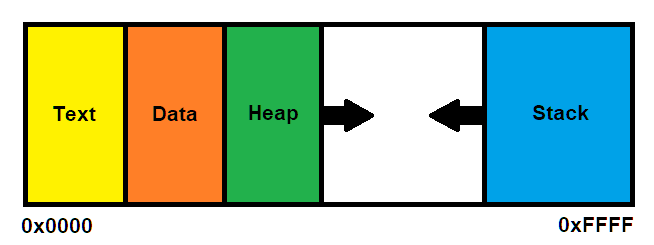
\includegraphics[width=0.7\textwidth,height=0.75\textheight,keepaspectratio]{images/process.png}
    \caption{Prozess im Speicher}
\end{figure}

Wenn eine Funktion aufgerufen wird, legt diese zunächst ihre Funktionsparameter auf den Stack,
gefolgt von einer Return-Adresse, die angibt, zu welcher Stelle im Programm im Anschluss an die
Ausführung der Funktion gesprungen wird, und einem Base Pointer. Darauf folgen lokale Daten,
die von der Funktion verwendet werden, wie z.\,B. ein Char Array.
\pagebreak
\subsection{Stack Overflow}
Der zuvor beschriebene Aufbau des Stacks lässt sich nun durch gezieltes Einfügen von Daten in eine Funktion ausnutzen.
Wenn beispielsweise ein Char Array mit einer Größe von 64 Bytes auf den Stack gelegt wird und es dem Angreifer gelingt,
als Folge von fehlerhafter Programmierung eine Zeichenkette mit mehr als 64 Bytes in das Array zu laden, so können
die überschüssigen Zeichen andere Daten im Stack überschreiben. Durch diese Methode kann der Prozess auf folgende
Weisen beeinflusst werden:
\begin{itemize}
    \item Es kann der Wert einer Variable verändert werden, um den Prozess zu manipulieren.
    \item Function Pointer können manipuliert werden, um den Programmfluss umzuleiten und zuvor präparierten Shellcode auszuführen.
    \item Auch durch das Überschreiben von Return Pointern kann auf Shellcode umgeleitet werden.
\end{itemize}

Ausgeführter Shellcode läuft dann immer unter denselben Privilegien wie der Prozess.
\begin{figure}[h]%
    \centering
    \subfloat[\centering Vorher]{{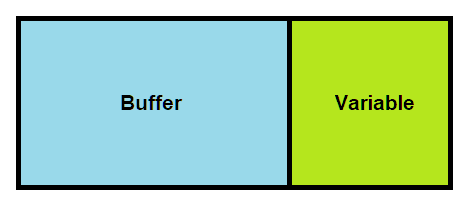
\includegraphics[width=0.45\textwidth,height=0.75\textheight,keepaspectratio]{images/buffer1.png} }}%
    \qquad
    \subfloat[\centering Nachher]{{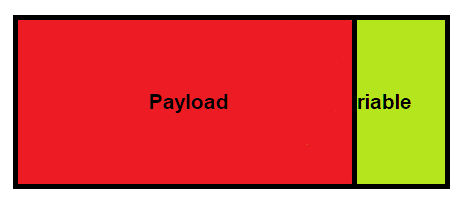
\includegraphics[width=0.45\textwidth,height=0.75\textheight,keepaspectratio]{images/buffer2.png} }}%
    \caption{Buffer im Stack während eines Overflows}%
    \label{fig:example}%
\end{figure}

\subsection{Heap Overflow}
Während der Laufzeit eines Programms allozierter Speicher (z.\,B. durch \codeline{malloc()}) wird im Heap angelegt. Dabei setzt sich 
jeder Speicherblock aus einem Header und dem tatsächlich angeforderten Speicher zusammen. Der Header enthält hierbei, 
je nach Implementation, Informationen über den Block, wie z.\,B. seine Größe. Aus diesen Informationen kann dann abgeleitet 
werden, an welcher Stelle der nächste Block beginnt.

Wenn ein Angreifer nun Manipulationen im Heap-Speicher vornehmen möchte, muss er die verwendete Implementation kennen 
und kann in der Regel nur in Richtung der neu allozierten Speicherblöcke überschreiben. Da er aus dem Heap keine Möglichkeit 
hat, Sprungadressen direkt zu manipulieren und den Programmfluss so umzuleiten, muss er versuchen, einen bestimmten 
Speicherblock zu überschreiben, zu dem im weiteren Programmverlauf noch einmal gesprungen wird. Dies macht Heap Overflows 
in der Praxis um einiges komplexer und schwieriger als Stack Overflows.

